\iffalse
The new generation of the collaborative robots allow the use of small robot arms working in an asynchronous or synchronous fashion with human workers.  Such an example of the collaborative robot is the YuMi robot, dual 7-DOF robot arms designed for precise manipulation of small parts better known in computer vision as rigid body. For further acceptance of such robots in the industry, some methods and sensors systems have to be developed to allow them to pick parts without the position of the part being known in advance, just as humans do.
This thesis is focused on the implementation of an algorithm for determing the positition of the known parts. We first deal with a robot-camera calibration, then  we propose a method to obtain the ground truth position of known parts. As step in between a 3D model of the known part needs to be created.
\fi


	\bibitem{planarTargets}
		B. Atcheson, F. Heide, and W. Heidrich,
		"CALTag: High Precision Fiducial Markers for CameraCalibration" in: Vision, Modeling, and Visualization, 2010, \url{https://pdfs.semanticscholar.org/2dba/e046717b058382a5a04f800405f92d040200.pdf}.






\begin{figure}[!h]
\begin{center}
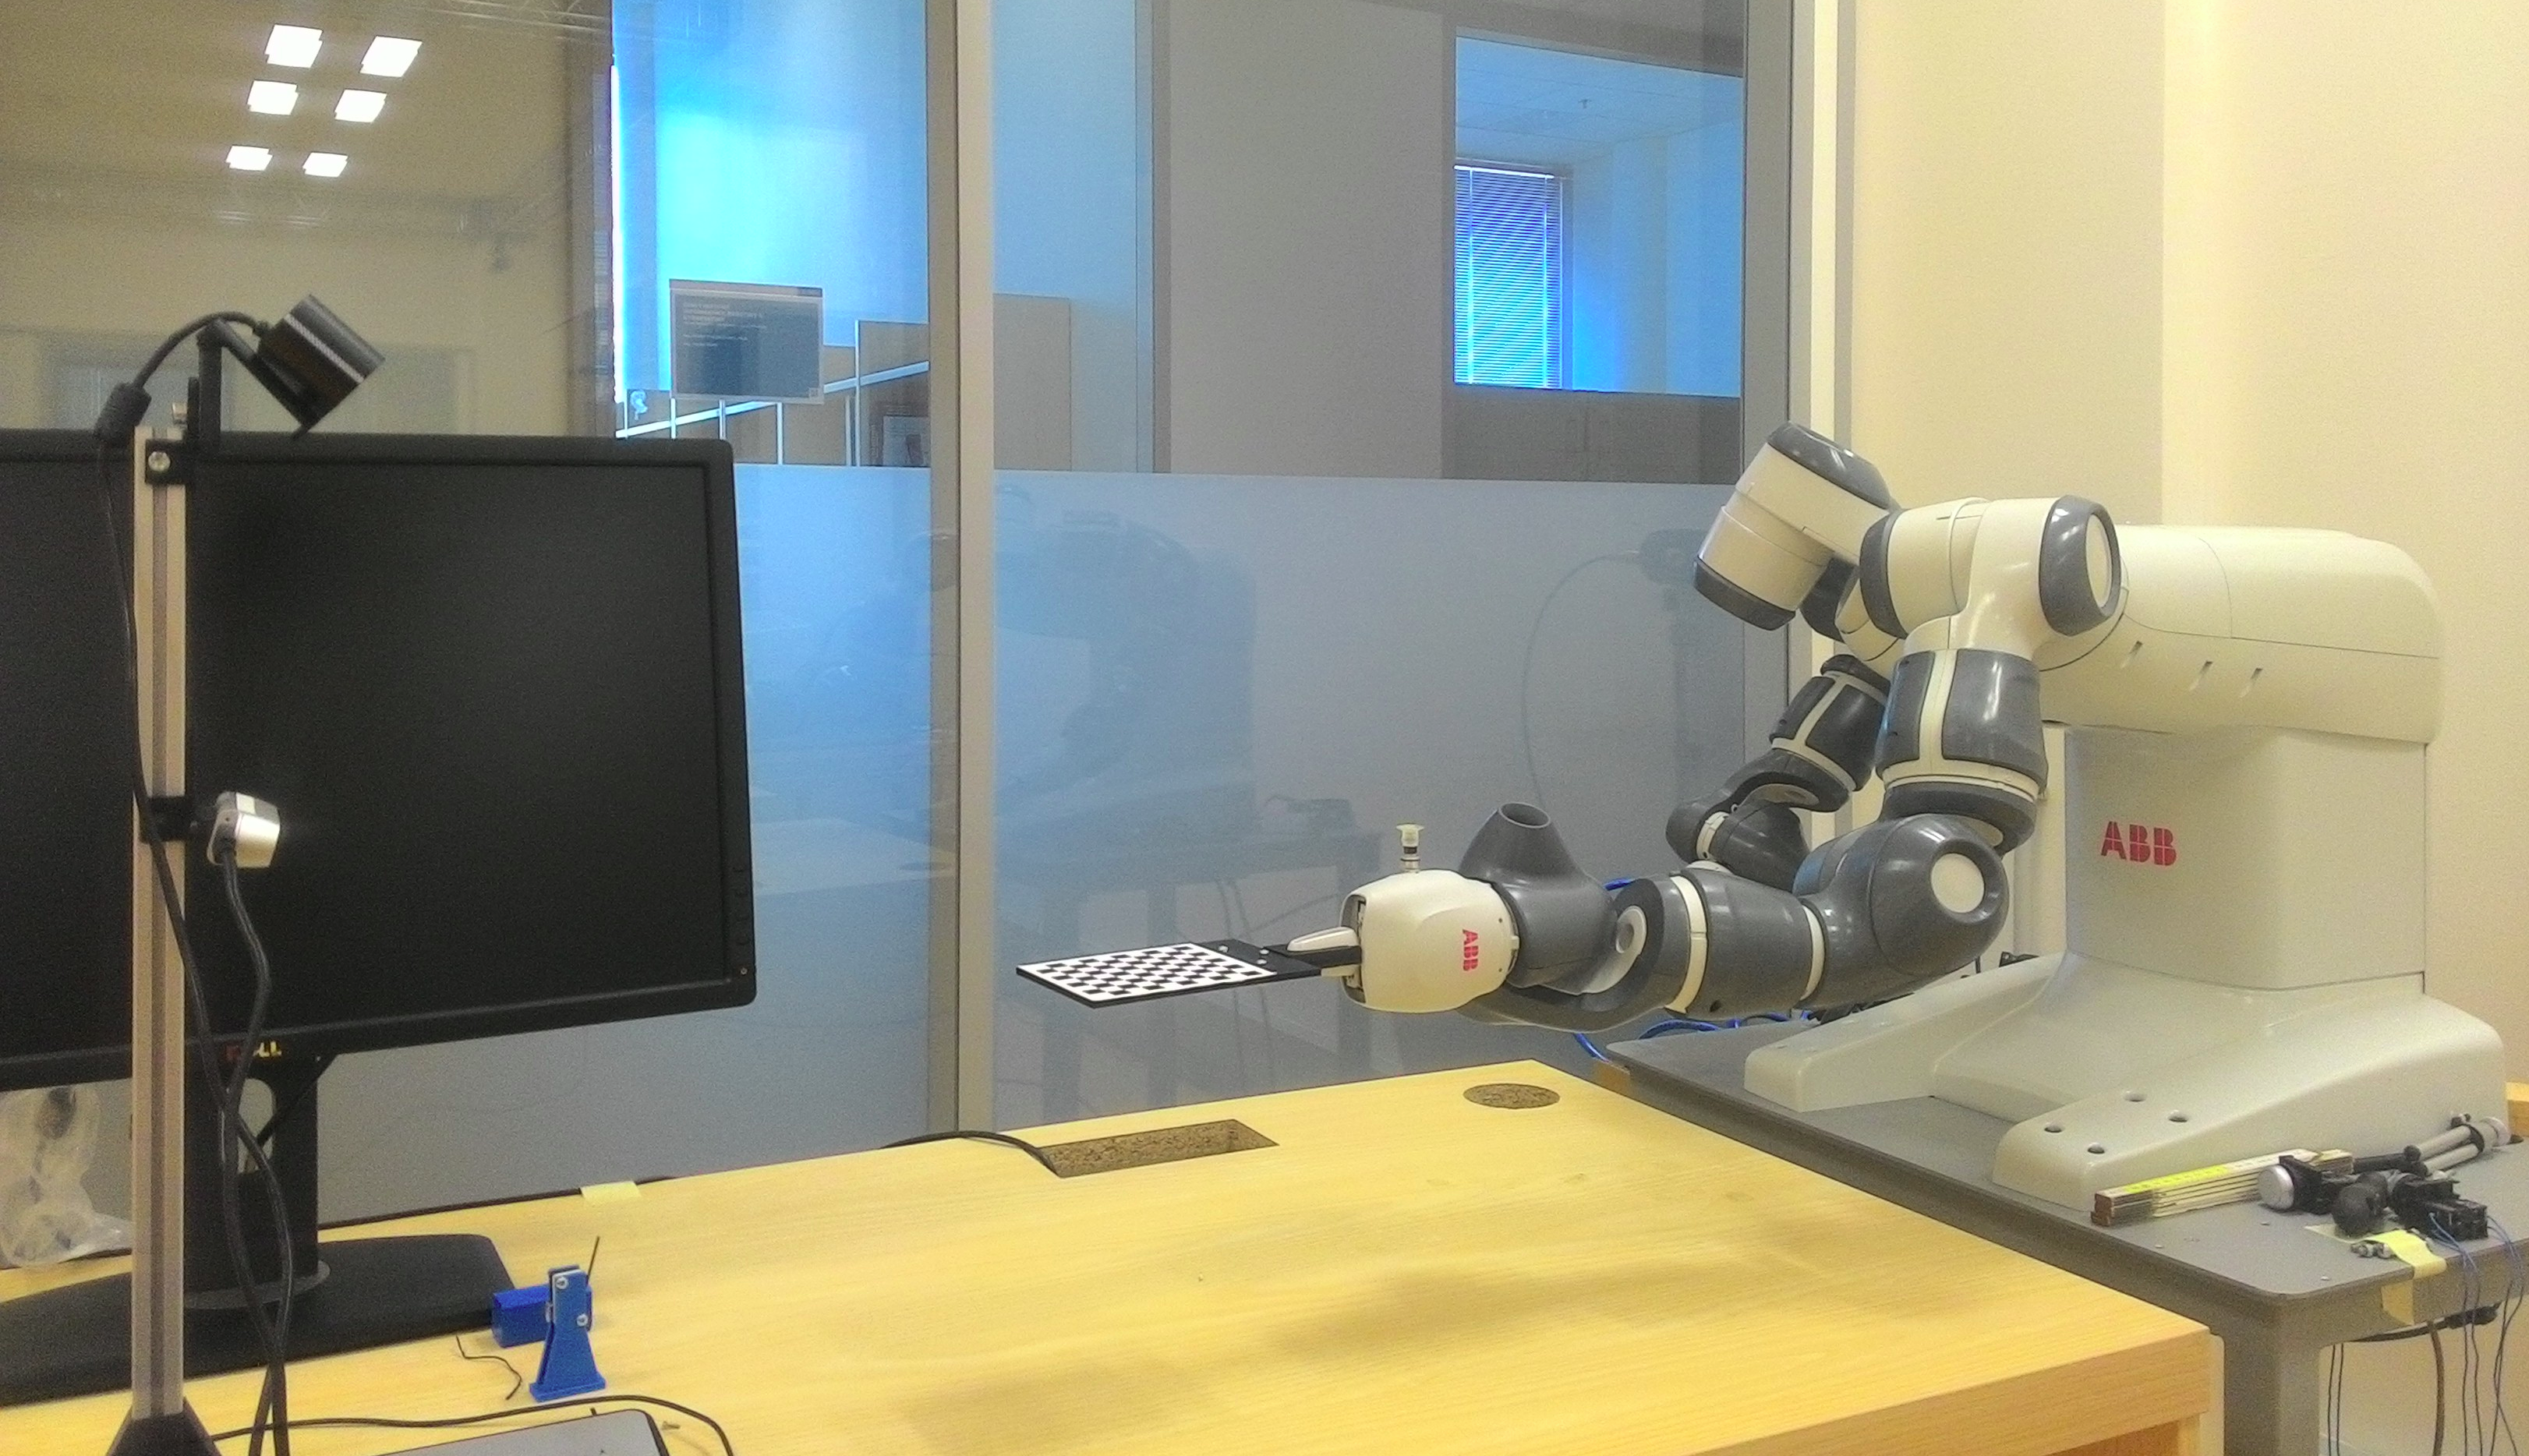
\includegraphics[width=4in]{figures03/setup.png}
\caption{Overview of the setup, a ABB YUMI robot with a gripper holding the calibration plate. The camera is fixed around the robot workspace and pointed at the checkerboard}%\cite{temp2}}
\label{fig:setup}
\end{center}
\end{figure}



In \ref{caltar} methods to estimate the position of the camera relative to a calibration targets have been briefly reviewed. This position data, plus the pose of calibration plate relative to the robot base frame are used to calculate the pose of the camera coordinate system relative to the robot base coordinate system with the help of TF ROS packages.




In Figure \ref{fig:setup} an example setup is given of a robot arm with a gripper holding a calibration plate with a the 6x9  checkerboard sticks on it. The robot arm can move the calibration plate around the robot workspace where a camera is fixed and takes a sequence of pictures from different movement.


%%%%%%%%%%%%%%%%%%%%%%%%%%%%%%%%%%%
\iffalse
%%% not yet
 The principle is that the checkerboard is detected, the pose of camera relative to the chessboard frame and the pose of the checkerboard relative to the robot frame is being streamed through the tf topic of  the ROS network, then a pose of the camera relative to the robot frame is retrieved with by using tf listening transform. This transformation is saved. The cycle repeats for each one of the movement the robot has to execute. The number of successful detection of the checkerboard is saved also. When the robot has completed all the movements, an average of all poses is computed. 

As to, the robot control, several packages from the open source community were tested with the idea in mind to interface the robot with a ros node.  Since the whole system was developed in ROS, which offers huge support to most of the sensors and robots, a rapid development can be done. 
With the two types of experiment to handle and how the communication with the robot is hold. 


\begin{itemize}
\item Internal camera calibration where a data collection is requiring.

\end{equation}
\item Eye-to-hand calibration where a robot move is requiring. 

\end{itemize}

The propose robot-camera calibration method was successfully performed provided that the checkerboard was detected by the 3D camera to be calibrated.


 Results are divided in two sections, each one requiring an independent set. For an intrinsic calibration, since the extrinsic calibration depends on the known intrinsic parameteres of the camera.  it is not required that the calibration plate be attached to the robot gripper. As to, the extrinsic calibration, the calibration target which is fixed on the customed-made plate is attached to the gripper of the robot.

\subsection{Dataset}

For the performance evaluation, a dataset of scenes was collected. It contains 60 point clouds wich can be classified as:
\begin{itemize}
\item point clouds, captured in a synthetic environment.
\item point clouds, captured in real environment. 
\end{itemize}

\subsection{Metrics}
In this thesis two standard metrics are used in order to evaluate the performance of the pose estimation algorithms.
\begin{itemize}
\item Precision:
\item point clouds, captured in real environment. 
\end{itemize}

\subsection{Testing environment}
The robot-camera calibration method as well as the pose estimation system were implemented in Python within ROS enviornment, making use of highly optimized libraries for 3D point cloud processing and tools. 

\subsection{Hardware}
All tests for which we report the expirements and result have been made using a personal computer Lenovo ThinkPad T430, Intel Core i5-3320 CPU 2.60GHz x 4, 7.8GB RAM, Ubuntu 16.04 64-bit OS
and ROS Kinetic release.

\fi
